% !TeX spellcheck = es_ES
%%%%%%%%%%%%%%%%%%%%%%%%%%%%%%%%%%%%%%%%%
% Stylish Article
% LaTeX Template
% Version 2.1 (1/10/15)
%
% This template has been downloaded from:
% http://www.LaTeXTemplates.com
%
% Original author:
% Mathias Legrand (legrand.mathias@gmail.com) 
% With extensive modifications by:
% Vel (vel@latextemplates.com)
% Final ACS by:
% Juan Barbosa
% License:
% CC BY-NC-SA 3.0 (http://creativecommons.org/licenses/by-nc-sa/3.0/)
%
%%%%%%%%%%%%%%%%%%%%%%%%%%%%%%%%%%%%%%%%%
\documentclass[fleqn,11pt]{SelfArx}
%\usepackage[superscript]{cite}
\usepackage{wrapfig}
\usepackage{rotating}
\usepackage{subcaption}
\usepackage[numbers, super]{natbib}
%----------------------------------------------------------------------------------------
%	ARTICLE INFORMATION
%----------------------------------------------------------------------------------------

\JournalInfo{Laboratorio Org\'anica III, No. 8, 5/12/2017} % Journal information
\Archive{ }

\PaperTitle{Oxidaci\'on de Bayer Villiger} %
%\Keywords{Keyword1 --- Keyword2 --- Keyword3} % Keywords - if you don't want any simply remove all the text between the curly brackets
%\newcommand{\keywordname}{Keywords} % Defines the keywords heading name

%----------------------------------------------------------------------------------------
%	ABSTRACT
%----------------------------------------------------------------------------------------

\Abstract{
	\begin{wrapfigure}{r}{0.5\textwidth}
		\centering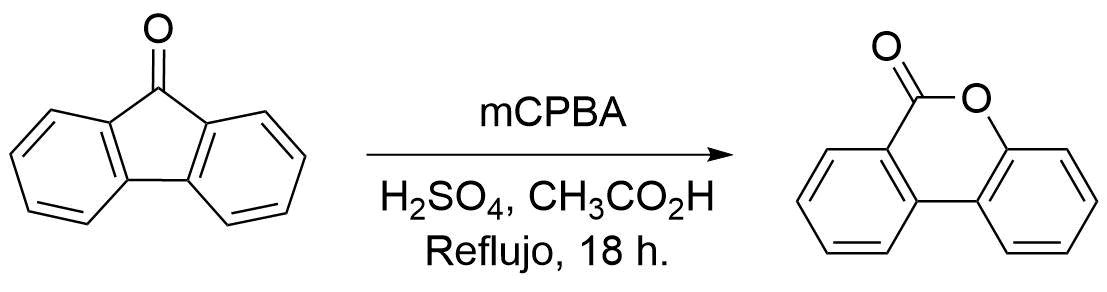
\includegraphics[width=\linewidth]{structures/reaction.png}
	\end{wrapfigure}
	La síntesis de 6H-benzo[c]cromen-6-ona se llevó a cabo por medio de la oxidación de Baeyer-Villiger de la fluorenona con mCPBA, ácido sulfúrico y ácido acético. El crudo de reacci\'on fue purificado en columna, obteniendo el producto con un porcentaje de recuperación del 71.2 \%. El producto fue elucidado por $^1$HRMN, $^{13}$CRMN, y un experimento DEPT-135.
}

%----------------------------------------------------------------------------------------

\begin{document}
	
	\flushbottom % Makes all text pages the same height
	
	\maketitle % Print the title and abstract box
	
	%\tableofcontents % Print the contents section
	
	\thispagestyle{empty} % Removes page numbering from the first page
	\renewcommand{\tablename}{Tabla} 
	
	
	%----------------------------------------------------------------------------------------
	%	ARTICLE CONTENTS
	%----------------------------------------------------------------------------------------
	
	\section*{Introducci\'on} % The \section*{} command stops section numbering
	%------------------------------------------------
	La 6H-benzo[c]cromen-6-ona hace parte de la familia de las cumarinas, las cuales se caracterizan por su aromaticidad, pues presentan un anillo arom\'atico sustitu\'ido por un grupo \'ester insaturado c\'iclico como se observa en el \autoref{sch:cumarina}.
	\begin{scheme}
		\centering
		\caption{Estructura de la cumarina en azul, en rojo el anillo funcionado siendo la molécula total una benzo[c]cumarina.}
		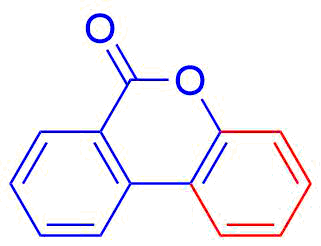
\includegraphics[width=0.35\linewidth]{structures/ascumarine.png}
		\label{sch:cumarina}
	\end{scheme}

	La familia de las cumarinas es de origen natural, siendo su fuente más común las plantas. Además si se tiene en cuenta que estas pueden presentar un anillo de benceno adicional, se obtiene una nueva familia conocida como las benzocumarinas. Esta nueva familia se subclasifica en cuatro estructuras bases dependiendo de la ubicación relativa del anillo fusionado, estos se muestran en el \autoref{sch:benzocumarinas}\cite{Kim2014}.
	\begin{scheme}
		\centering
		\caption{(a) benzo[c]cumarina, (b) benzo[h]cumarina, (c) benzo[h]cumarina, (d) benzo[g]cumarina.}
		\begin{tabular}{cc}
			\begin{subfigure}[h]{0.45\linewidth}
				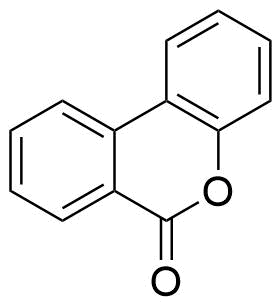
\includegraphics[width=0.5\linewidth]{structures/cbenzo.png}
				\caption{}
			\end{subfigure} &
			\begin{subfigure}[h]{0.45\linewidth}
				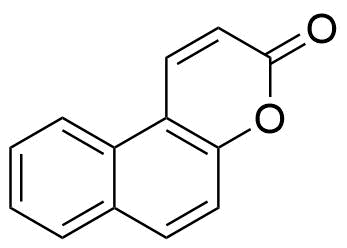
\includegraphics[width=0.7\linewidth]{structures/hbenzo.png}
				\caption{}
			\end{subfigure} \\
			\begin{subfigure}[h]{0.45\linewidth}
				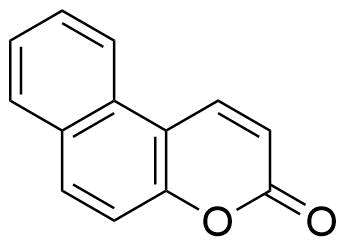
\includegraphics[width=0.6\linewidth]{structures/fbenzo.png}
				\caption{}
			\end{subfigure} &
			\begin{subfigure}[h]{0.45\linewidth}
				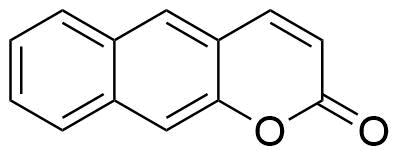
\includegraphics[width=0.8\linewidth]{structures/gbenzo.png}
				\caption{}
			\end{subfigure}
		\end{tabular}
		\label{sch:benzocumarinas}
	\end{scheme}

	Para el caso específico de la benzo[c]cumarina, se tiene que el método más usado en su síntesis en la oxidación de Baeyer-Villiger, siendo esta una reacción en la que una cetona es oxidada para la obtención de un ester. Dependiendo de la naturaleza de la cetona, se pueden obtener esteres alifáticos o lactonas, mediante el uso de peroxiacidos\cite{EJOC:EJOC737,CHIR:CHIR39}.
	
	En el contexto de la medicina las cumarinas son usadas como antocoagulantes, antioxidante, antibacterial, antiinflamatoria, antifúngica y antimicrobiana\cite{Kim2014}. Así mismo las benzocumarinas presentan actividad como antiinflamatorios\cite{doi:10.1021/ol400877q}.
	
	Todas las benzocumarinas presentan algún grado de aromaticidad, lo que hace que tengan una naturaleza propia de los sistemas con electrones $\pi$, en ese sentido muchas de estas han sido usadas en el desarrollo de marcadores fluorescentes para tejidos biológicos\cite{Kim2014}.
	
	Para esta práctica se realizará la síntesis de la 6H-benzo[c]cromen-6-ona a partir de fluorenona y mCPBA, en presencia de ácido acético y ácido sulfúrico.
	
	\section{Resultados y Discusi\'on}
	
	El mecanismo de la reacción se divide en 4 pasos\cite{Li2014}. El primero es la protonación del ácido acético en presencia de un ácido fuerte como el ácido sulfúrico, lo cual se ve favorecido por la presencia de agua en el medio.
	\begin{scheme}
		\centering
		\caption{Protonación del ácido acético.}
		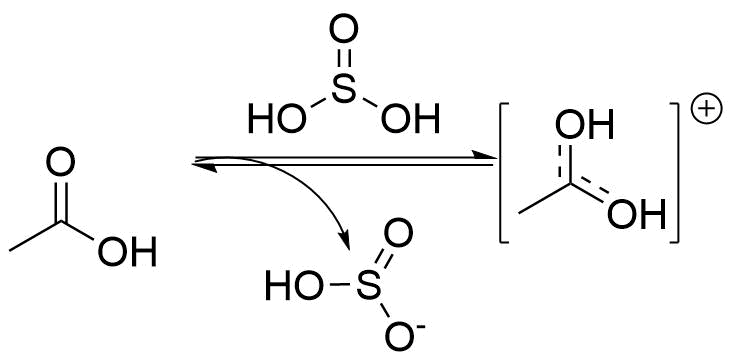
\includegraphics[width=0.6\linewidth]{structures/protonation.png}
	\end{scheme}

	Posteriormente tiene lugar el ataque nucleofílico de la fluorenona \textbf{(a)}, el cual da lugar a un catión sobre la molécula, este catión si bien se ubica sobre el oxígeno, está estabilizado por la estructura resonante.
	\begin{scheme}
		\centering
		\caption{Protonación de la fluorenona.}
		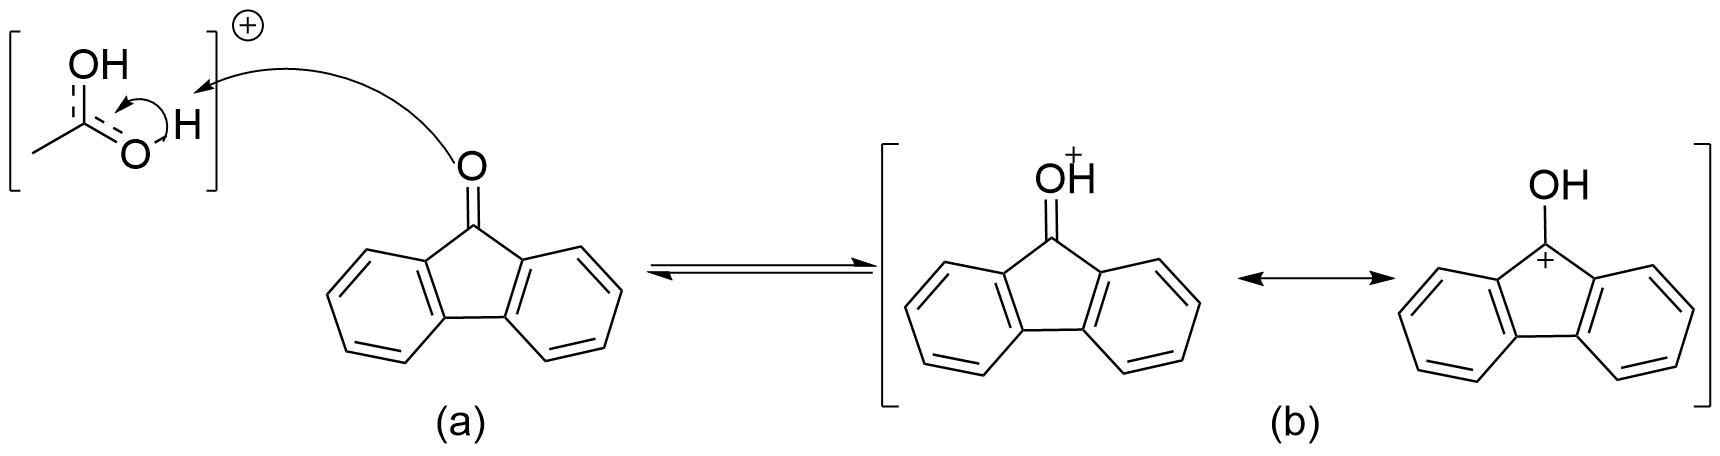
\includegraphics[width=\linewidth]{structures/flourenoneprotonation.png}
	\end{scheme}
	
	Tras darse la protonación de la flourenona, se promueve el ataque nucleofílico del mCPBA a al carbono carbonílico, dando lugar al intermediario de Criegee\cite{Alvarez-Idaboy2006}.
	\begin{scheme}
		\centering
		\caption{Formación del intermediario de Criegee\cite{Alvarez-Idaboy2006}.}
		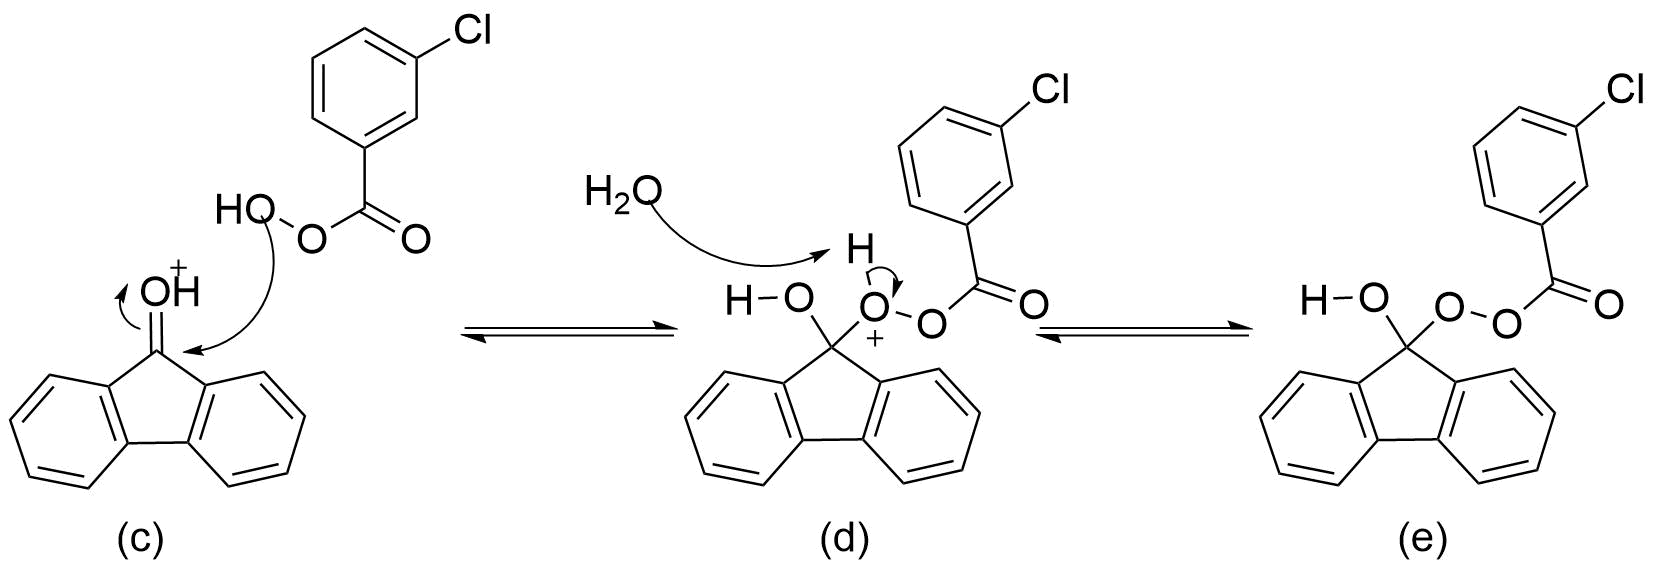
\includegraphics[width=\linewidth]{structures/Criegee.png}
	\end{scheme}

	El paso final de la reacción es la formación de la benzocumarina, el cual se da de manera concertada entre el ácido acético y el intermediario de Criegee. El oxígeno del carbonilo de la molécula de Criegee ataca el protón del ácido acético, de manera análoga el oxígeno del carbonilo del ácido ataca el grupo hidroxi del intermediario, el enlace \ce{O-H} se rompe y el par electrónico involucrado da lugar a la formación de un carbonilo. Finalmente y con la formación del carboxilo tiene lugar la formación del enlace oxígeno-grupo fenilo.
	\newpage
	\begin{scheme}
		\centering
		\caption{Formación de la benzocumarina.}
		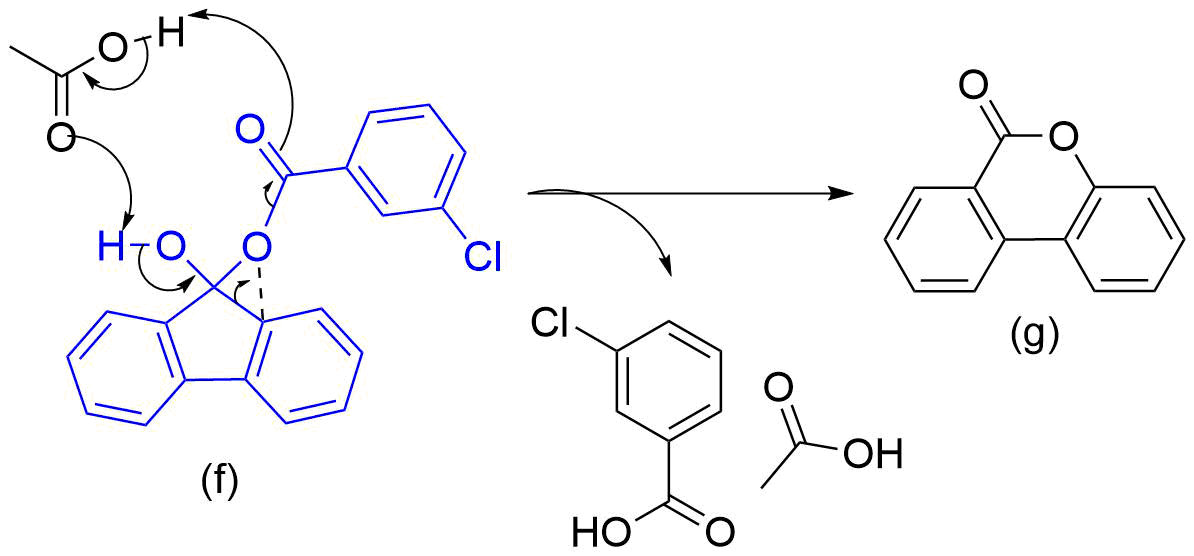
\includegraphics[width=0.7\linewidth]{structures/final.png}
	\end{scheme}

	La caracterización del producto se llevó a cabo usando $^{1}$HRMN, $^{13}$CRMN, y un experimento DEPT. En el caso del estudio de protones fue posible asignar 7 señales de las 8 que se esperan para la molécula, sin embargo la integral para una de las señales es propia de dos protones, por lo cual se argumenta que estas están solapadas.
	\begin{figure}[h]
		\centering
		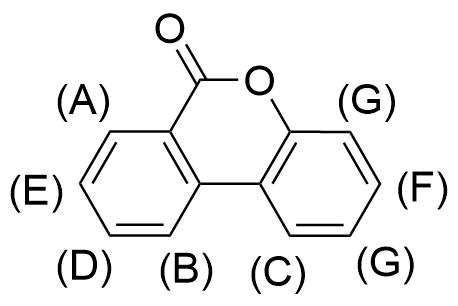
\includegraphics[width=0.5\linewidth]{structures/H.png}
		\caption{Asignación de señales de $^{1}$HRMN.}
		\label{fig:hrmn}
	\end{figure}

	Como se observa en la \autoref{fig:hrmn}, todas las señales esperadas se encuentran en la región aromática, aquellas que se encuentran más desprotegidas corresponden con \textbf{(A)}, \textbf{(B)} y \textbf{(C)}, siendo la primera la que presenta menor densidad electrónica debido a que se encuentra en la posición \textit{orto} a la cetona, esta señal se observa a 8.40 ppm. Posteriormente se observan las señales de las posiciones \textbf{(B)} y \textbf{(C)} las cuales presentan una densidad electrónica algo menor debido a su interacción con el anillo vecino. Todas estas tres señales presentan multiplicidad de dobletes, dado que cada una observa un hidrógeno vecino. Posteriormente se encuentran las señales del anillo izquierdo, el cual se encuentra más cerca a la cetona y por ende, con menor densidad electrónica. La posición \textit{para} se encuentra más desprotegida, puesto que está más activada. La multiplicidad de estas señales es triplete. A campo más alto se encuentran las señales del anillo derecho, en el caso de las señales \textbf{(G)} se observa un multiplete dado que no fue posible segregar la información de cada protón. La señal a menor frecuencia corresponde entonces con \textbf{(F)}, la cual se presenta como triplete. Las señales observadas en el RMN corresponden con las reportadas en la literatura\cite{doi:10.1021/ol400877q}.	
	\newpage
	
	Ahora bien, es importante resaltar que el número de señales muestra que la reacción tuvo lugar, dado que para el reactivo de partida se esperan únicamente 4 señales por la simetría de la misma, teniendo en cuenta que se observan 7, con los valores esperados para las integrales se tiene la confirmación del producto. Adicionalmente en los espectros RMN de carbono se observan cuatro nuevas señales correspondientes a los carbonos cuaternarios de los anillos fusionados y el carbonilo. Estas últimas dejan de observarse en el experimento DEPT, confirmando su naturaleza de carbonos cuaternarios, adicional a esto el experimento DEPT no muestra ninguna señal de carbonos secundarios, lo cual es de esperar para la molécula objetivo.
	
	\section{Conclusiones}
	Se consiguió sintetizar la 6H-benzo[c]cromen-6-ona por medio de una oxidación de Baeyer-Villiger con Ácido meta-cloroperbenzoico, ácido acético y ácido sulfúrico. Los espectros de RMN $^1$H, $^{13}$C y $^{13}$C DEPT, permitieron elucidar el producto, sin embargo se observan algunas señales en la región alinfática, por lo cual no es posible reportar el rendimiento y únicamente se habla de recuperación del 71.2 \%. 
	\section{Secci\'on experimental}
	En un balón de reacción fueron disueltos 0.9035 g de fluorenona (5.0 mmol) y 1.9017 g (7.5 mmol) de mCPBA en 10 mL de ácido acético y 2 mL de ácido sulfúrico concentrado (37.5 mmol). El balón fue llevado a reflujo por 18 horas. Una vez terminado este tiempo la mezcla fue enfriada a temperatura ambiente, y posteriormente fueron adicionados 100 mL de éter etílico y 100 mL de \ce{Na2S2O3} para destruír el exceso de peróxido, mediante agitación constante por 1 hora. A la mezcla resultante se le realiza una extracción líquido-líquido, de la cual se obtiene la fase orgánica que posteriormente es lavada con una solución saturada de bicarbonato de sodio y agua. La fase orgánica se seca con sulfato de magnesio y el disolvente se retira a presión reducida. El producto es purificado por cromatografía de columna usando fase móvil: acetato-pentano (3:7).
	\paragraph{6H-benzo[c]cromen-6-ona:}
	$^1$H NMR (400 MHz, \ce{CDCl3}) $\delta$ 8.40 (d, J = 7.9 Hz, 2H), 8.10 (d, J = 9.1 Hz, 2H), 8.06 (d, 2H), 7.83 (t, 2H), 7.59 (t, J = 11.1, 4.1 Hz, 2H), 7.48 (t, J = 10.0, 4.1 Hz, 3H), 7.40 – 7.30 (m, J = 14.8, 7.7, 4.3 Hz, 4H).
	
	$^{13}$C NMR (101 MHz, \ce{CDCl3}) $\delta$ 134.80 (s), 130.53 (s), 129.00 (s), 124.45 (s), 122.79 (s), 121.71 (s), 120.33 (s), 117.79 (s).
	
	
	%----------------------------------------------------------------------------------------
	%	REFERENCE LIST
	%----------------------------------------------------------------------------------------
	\phantomsection
	\bibliography{informe}
	\bibliographystyle{achemso}
	
	%----------------------------------------------------------------------------------------
	\onecolumn
	\section{Informaci\'on suplementaria}\label{sec: complementaria}
	
	\rotatebox{90}
	{
		\begin{minipage}{0.9\textheight}
			\centering
			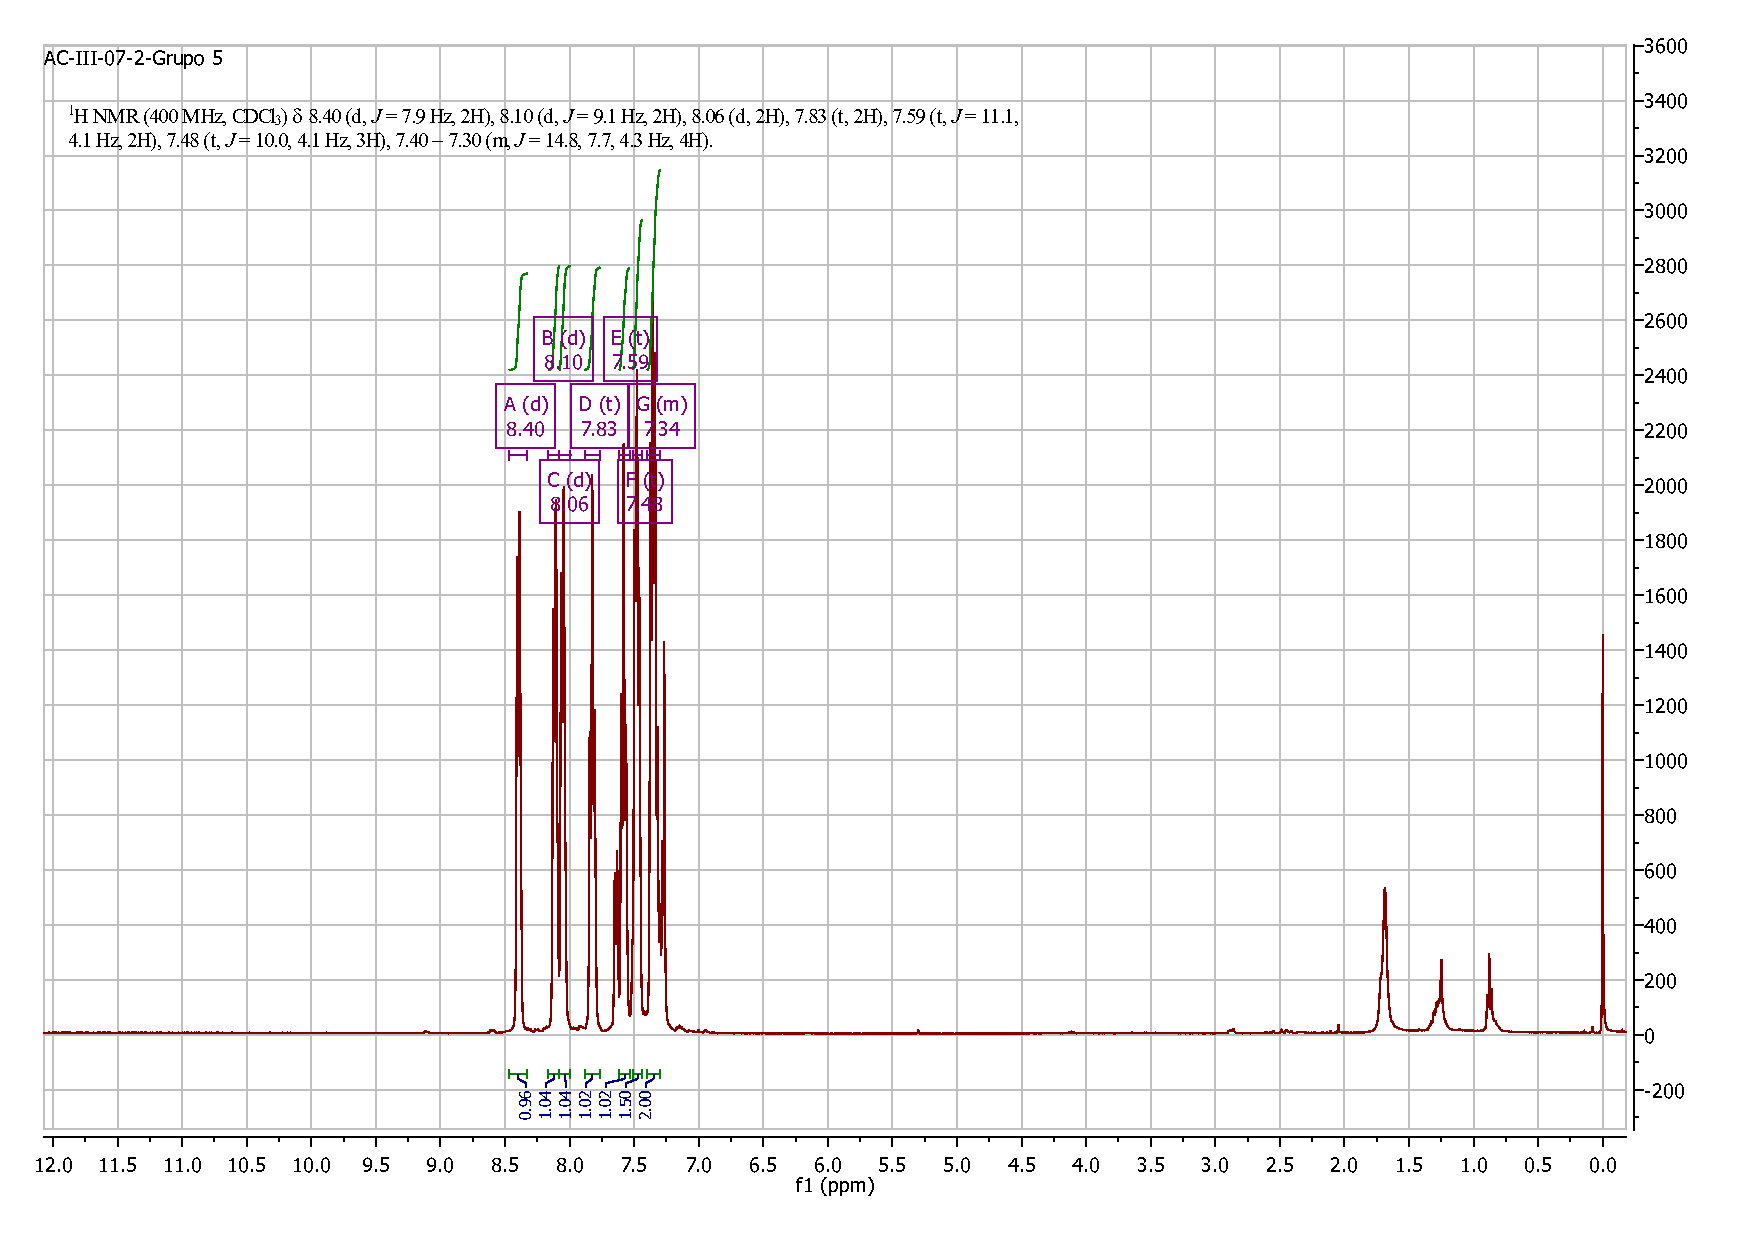
\includegraphics[height=0.65\textheight]{RMN/HRMN.pdf}
			\captionof{figure}{$^1$HRMN del producto.}
			\label{HRMN}
		\end{minipage}
	}

	\rotatebox{90}
	{
		\begin{minipage}{0.9\textheight}
			\centering
			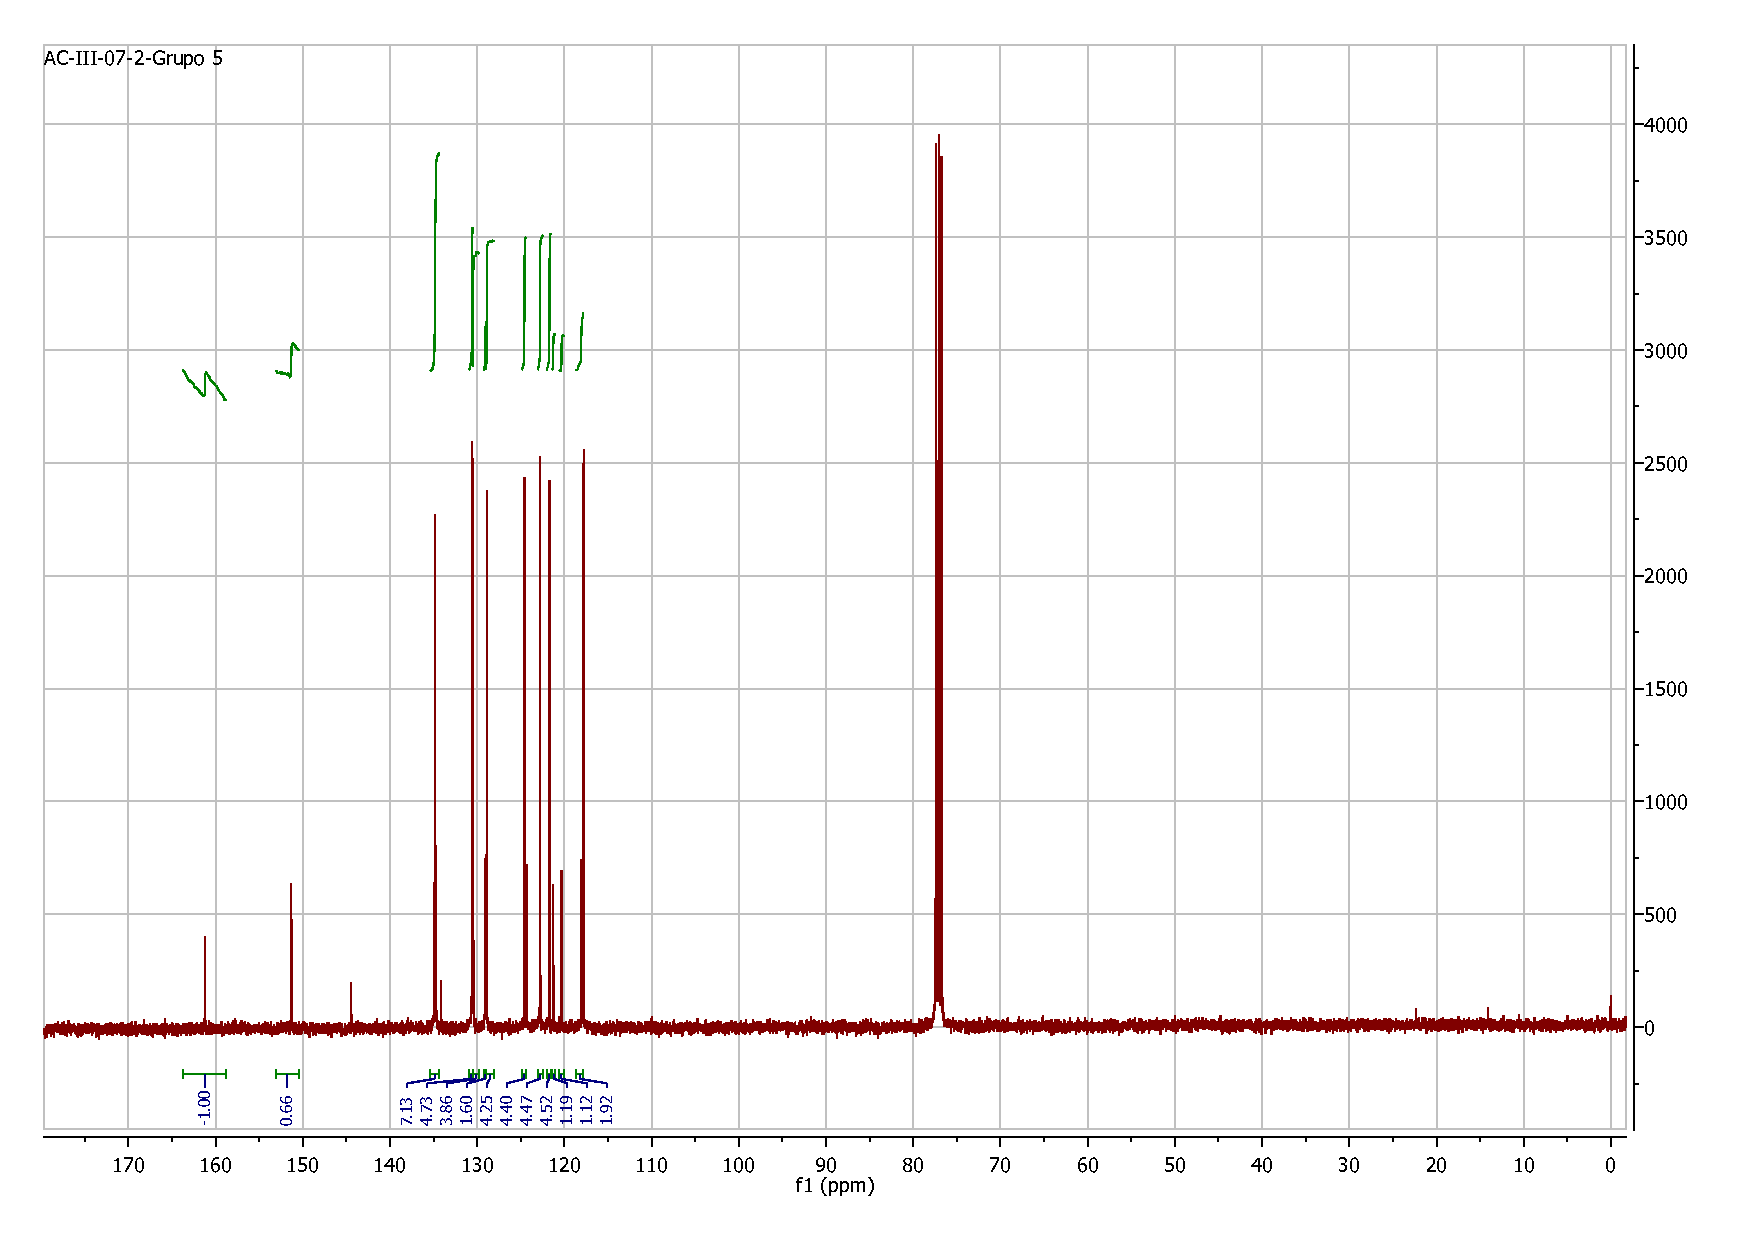
\includegraphics[height=0.65\textheight]{RMN/CRMN.pdf}
			\captionof{figure}{$^{13}$CRMN del producto.}
			\label{CRMN}
		\end{minipage}
	}

	\rotatebox{90}
	{
		\begin{minipage}{0.9\textheight}
			\centering
			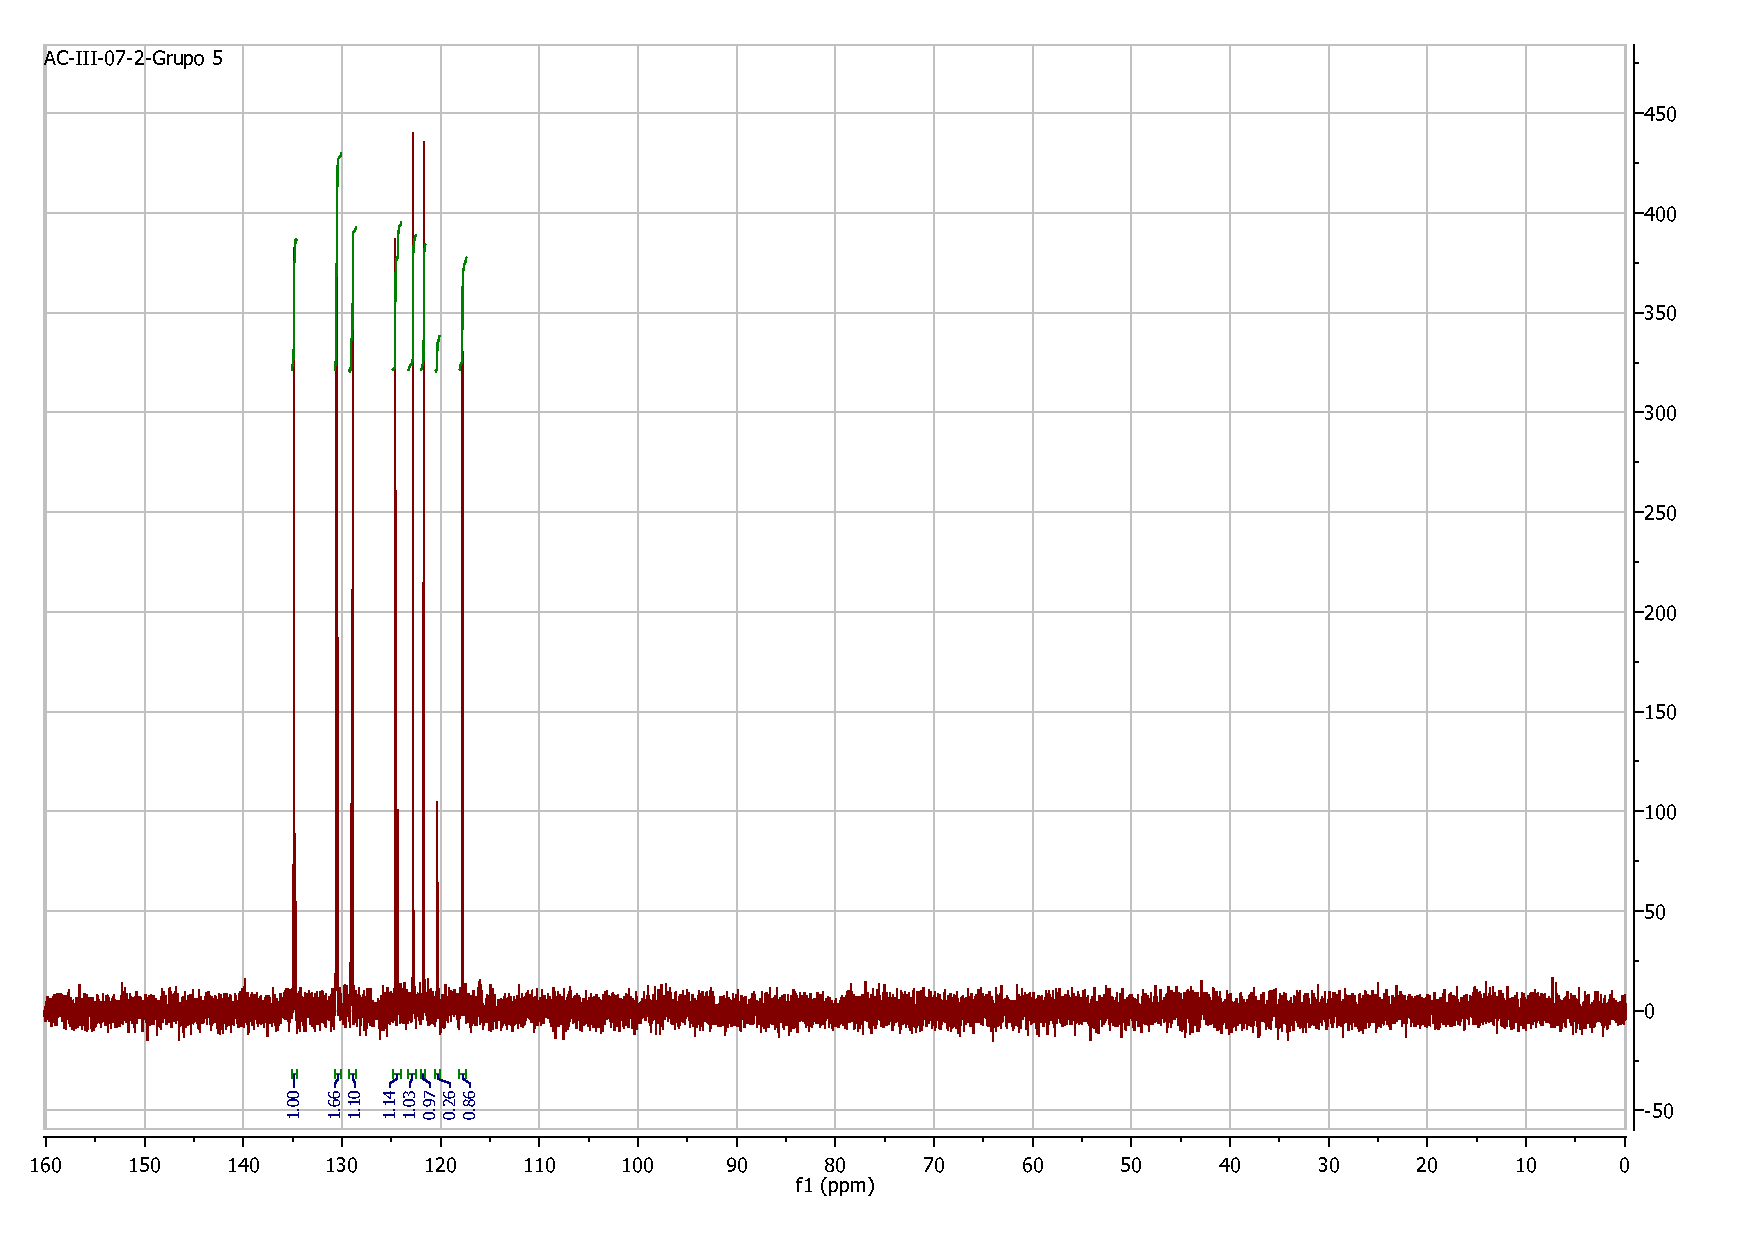
\includegraphics[height=0.65\textheight]{RMN/DEPT135.pdf}
			\captionof{figure}{Experimento DEPT-135 del producto.}
			\label{DEPT}
		\end{minipage}
	}
	
\end{document}